\documentclass[a4paper, 11pt]{article}

\usepackage{forest} 

\usepackage{soul}
\usepackage{xcolor}
\usepackage{graphicx}
\usepackage{multicol}

\usepackage{amsmath}

\usepackage{array}   % for \newcolumntype macro
\newcolumntype{L}{>{$}l<{$}} % math-mode version of "l" column type

\usepackage[hidelinks]{hyperref} 

% Poles settings:
\usepackage[left=15mm, top=10mm, right=15mm, bottom=10mm, head=5mm, foot=9mm]{geometry}

\usepackage{fontspec}
\setmainfont{FreeSerif}
\setsansfont{FreeSans}
\setmonofont{FreeMono}

% Polyglossia:
\usepackage{polyglossia}
\setdefaultlanguage{russian}
\newfontfamily\cyrillicfont{FreeSerif}[Script=Cyrillic]

\newcommand{\nx}[1]{\neg{x}_{#1}}
\newcommand{\x}[1]{x_{#1}}
\newcommand{\nphi}[0]{\overline{\varphi}}
\newcommand{\pirs}[2]{#1\downarrow#2}
\renewcommand{\phi}[0]{\varphi}
\renewcommand{\neg}[1]{\overline{#1}}

\makeatother

\begin{document}
\Large
\thispagestyle{empty}
\begin{center}
Министерство науки и высшего образования Российской Федерации \\
Федеральное государственное автономное образовательное учреждение высшего образования \\
«Национальный исследовательский университет ИТМО» \\
\vspace{1em}
\textsl{Факультет Программной Инженерии и Компьютерной Техники}\\
\end{center}

\vspace{1em}

\thispagestyle{empty}
\begin{center}

\includegraphics[width=8cm]{imgs/itmo.jpg}
\end{center}

\vspace{3em}

\begin{center}
\large{
\textsc{\textbf{
Лабораторная работа №3  \linebreak 
Выполнение циклических программ \linebreak 
Вариант №3118 \linebreak
}}
}
\end{center}

\vspace{10em}

\input{private.tex}

\newbox{\lbox}
\savebox{\lbox}{\hbox{\studName\hfill}}
\newlength{\maxl}
\setlength{\maxl}{\wd\lbox}
\hfill\parbox{10cm}{
\hspace*{5cm}\hspace*{-5cm}Студент:\hfill\hbox to\maxl{\studName\hfill}\\
\hspace*{5cm}\hspace*{-5cm}Преподаватель:\hfill\hbox to\maxl{\teacherName}\\
\\
\hspace*{5cm}\hspace*{-5cm}Группа:\hfill\hbox to\maxl{\groupNumber}\\
}

\vspace{\fill}

\begin{center}
Санкт-Петербург \\2021
\end{center}
\newpage

\tableofcontents
\vspace{2em}
\pagebreak{}

\section{Первая часть}
% 1.2. Представление булевой функции в аналитическом виде
% 1.3. Минимизация булевой функции методом Квайна–МакКласки
% 1.4. Минимизация булевой функции на картах Карно
% 1.5. Преобразование минимальных форм булевой функции
% 1.6. Синтез комбинационных схем в булевом базисе
% 1.7. Синтез комбинационных схем в универсальных базисах

\subsection{Составление таблицы истинности}
\begin{table}[h!]
  \centering
  \begin{tabular}{|L|L|}
    \hline
    \text{Условия, при которых} f = 1 & \text{Условия, при которых} f = d \\ \hline
    (x_1 x_2+x_3 x_4 x_5)=0, 5, 6, 7, 8 &  (x_3 x_4 x_5)=4 \\ \hline
  \end{tabular}
\end{table}

\begin{table}[h!]
  \centering
  \begin{tabular}{|c|c|c|c|c|c|c|c|}
  \hline
  N  & $x_1 x_2 x_3 x_4 x_5$ & $x_1 x_2$ & $(x_1 x_2)_{10}$ & $x_3 x_4 x_5$ & $(x_3 x_4 x_5)_{10}$ & +  & F  \\ \hline
  0  & 00000                 & 00        & 0                & 000           & 0                   & 0  & 1  \\ \hline
  1  & 00001                 & 00        & 0                & 001           & 1                   & 1  & 0  \\ \hline
  2  & 00010                 & 00        & 0                & 010           & 2                   & 2  & 0  \\ \hline
  3  & 00011                 & 00        & 0                & 011           & 3                   & 3  & 0  \\ \hline
  4  & 00100                 & 00        & 0                & 100           & 4                   & 4  & d  \\ \hline
  5  & 00101                 & 00        & 0                & 101           & 5                   & 5  & 1  \\ \hline
  6  & 00110                 & 00        & 0                & 110           & 6                   & 6  & 1  \\ \hline
  7  & 00111                 & 00        & 0                & 111           & 7                   & 7  & 1  \\ \hline
  8  & 01000                 & 01        & 1                & 000           & 0                   & 1  & 0  \\ \hline
  9  & 01001                 & 01        & 1                & 001           & 1                   & 2  & 0  \\ \hline
  10 & 01010                 & 01        & 1                & 010           & 2                   & 3  & 0  \\ \hline
  11 & 01011                 & 01        & 1                & 011           & 3                   & 4  & 0  \\ \hline
  12 & 01100                 & 01        & 1                & 100           & 4                   & 5  & d  \\ \hline
  13 & 01101                 & 01        & 1                & 101           & 5                   & 6  & 1  \\ \hline
  14 & 01110                 & 01        & 1                & 110           & 6                   & 7  & 1  \\ \hline
  15 & 01111                 & 01        & 1                & 111           & 7                   & 8  & 1  \\ \hline
  16 & 10000                 & 10        & 2                & 000           & 0                   & 2  & 0  \\ \hline
  17 & 10001                 & 10        & 2                & 001           & 1                   & 3  & 0  \\ \hline
  18 & 10010                 & 10        & 2                & 010           & 2                   & 4  & 0  \\ \hline
  19 & 10011                 & 10        & 2                & 011           & 3                   & 5  & 1  \\ \hline
  20 & 10100                 & 10        & 2                & 100           & 4                   & 6  & d  \\ \hline
  21 & 10101                 & 10        & 2                & 101           & 5                   & 7  & 1  \\ \hline
  22 & 10110                 & 10        & 2                & 110           & 6                   & 8  & 1  \\ \hline
  23 & 10111                 & 10        & 2                & 111           & 7                   & 9  & 0  \\ \hline
  24 & 11000                 & 11        & 3                & 000           & 0                   & 3  & 0  \\ \hline
  25 & 11001                 & 11        & 3                & 001           & 1                   & 4  & 0  \\ \hline
  26 & 11010                 & 11        & 3                & 010           & 2                   & 5  & 1  \\ \hline
  27 & 11011                 & 11        & 3                & 011           & 3                   & 6  & 1  \\ \hline
  28 & 11100                 & 11        & 3                & 100           & 4                   & 7  & d  \\ \hline
  29 & 11101                 & 11        & 3                & 101           & 5                   & 8  & 1  \\ \hline
  30 & 11110                 & 11        & 3                & 110           & 6                   & 9  & 0  \\ \hline
  31 & 11111                 & 11        & 3                & 111           & 7                   & 10 & 0  \\   \hline
  \end{tabular}
\end{table}
\subsection{Представление булевой функции в аналитическом виде}
\text{КДНФ:} $ f = \
\nx{1}\nx{2}\nx{3}\nx{4}\nx{5} \vee \
\nx{1}\nx{2}\x {3}\nx{4}\x {5} \vee \
\nx{1}\nx{2}\x {3}\x {4}\nx{5} \vee \
\nx{1}\nx{2}\x {3}\x {4}\x {5} \vee \
\nx{1}\x {2}\x {3}\nx{4}\x {5} \vee \
\nx{1}\x {2}\x {3}\x {4}\nx{5} \vee \
\nx{1}\x {2}\x {3}\x {4}\x {5} \vee \
\x {1}\nx{2}\nx{3}\x {4}\x {5} \vee \
\x {1}\nx{2}\x {3}\nx{4}\x {5} \vee \
\x {1}\nx{2}\x {3}\x {4}\nx{5} \vee \
\x {1}\x {2}\nx{3}\x {4}\nx{5} \vee \
\x {1}\x {2}\nx{3}\x {4}\x {5} \vee \
\x {1}\x {2}\x {3}\nx{4}\x {5}  \
$

ККНФ: $ f = \
(\x {1} \vee \x {2} \vee \x {3} \vee \x {4} \vee \nx{5})
(\x {1} \vee \x {2} \vee \x {3} \vee \nx{4} \vee \x {5})
(\x {1} \vee \x {2} \vee \x {3} \vee \nx{4} \vee \nx{5})
(\x {1} \vee \nx{2} \vee \x {3} \vee \x {4} \vee \x {5})
(\x {1} \vee \nx{2} \vee \x {3} \vee \x {4} \vee \nx{5})
(\x {1} \vee \nx{2} \vee \x {3} \vee \nx{4} \vee \x {5})
(\x {1} \vee \nx{2} \vee \x {3} \vee \nx{4} \vee \nx{5})
(\nx{1} \vee \x {2} \vee \x {3} \vee \x {4} \vee \x {5})
(\nx{1} \vee \x {2} \vee \x {3} \vee \x {4} \vee \nx{5})
(\nx{1} \vee \x {2} \vee \x {3} \vee \nx{4} \vee \x {5})
(\nx{1} \vee \x {2} \vee \nx{3} \vee \nx{4} \vee \nx{5})
(\nx{1} \vee \nx{2} \vee \x {3} \vee \x {4} \vee \x {5})
(\nx{1} \vee \nx{2} \vee \x {3} \vee \x {4} \vee \nx{5})
(\nx{1} \vee \nx{2} \vee \nx{3} \vee \nx{4} \vee \x {5})
(\nx{1} \vee \nx{2} \vee \nx{3} \vee \nx{4} \vee \nx{5})
$ \\\\


\subsection{Минимизация булевой функции методом Квайна–МакКласки}
\begin{center}
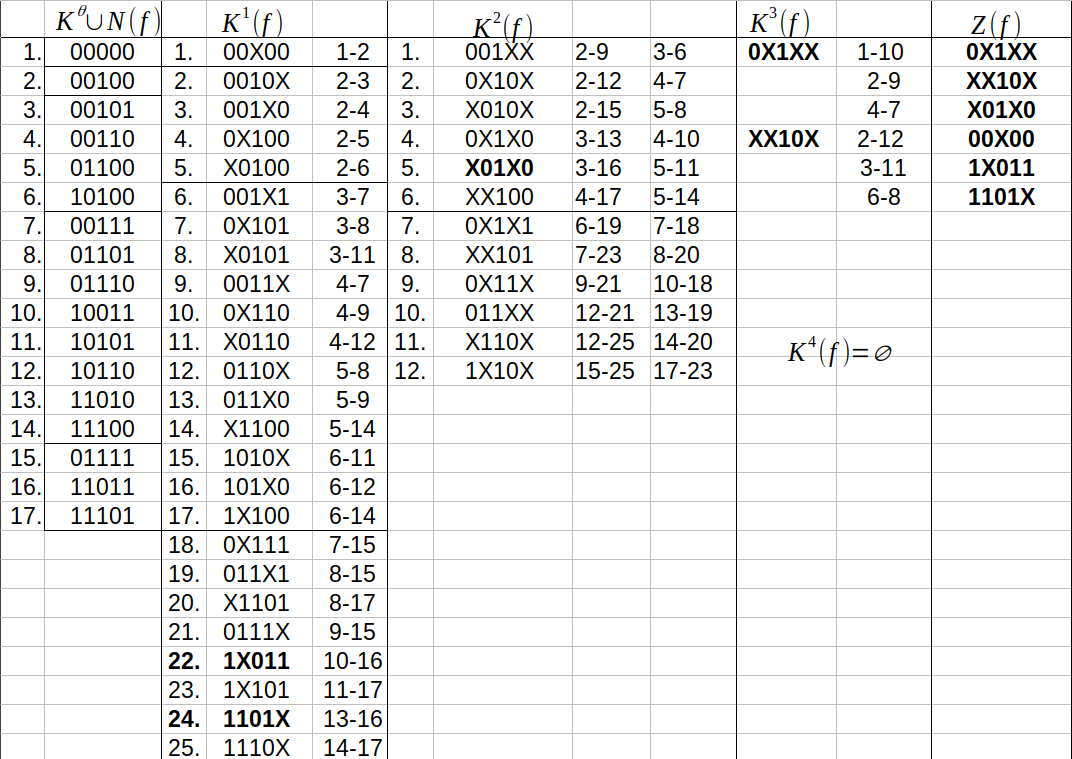
\includegraphics[width=\linewidth]{imgs/kvain_mak_table.png}
\end{center}
\par\textit{Составление импликантной таблицы}

Импликантная таблица в первоначальном виде содержит 6 строк (по числу 
простых импликант) и 13 столбцов (по числу существенных вершин).

\begin{center}
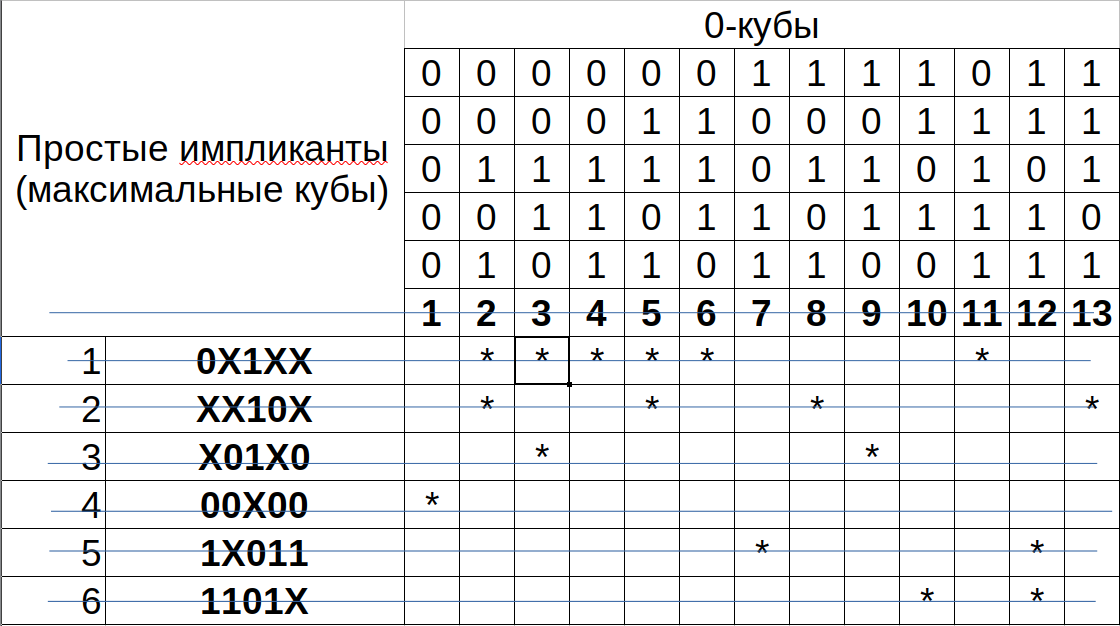
\includegraphics[width=0.6\linewidth]{imgs/implicant_table.png}
\end{center}

Все существенные вершины покрываются покрываются существенными импликантами.
\begin{equation*}
  C_{min}(f)= 
  \begin{Bmatrix}
    0 & X & 1 & X & X \\
    X & X & 1 & 0 & X \\
    X & 0 & 1 & X & 0 \\ 
    0 & 0 & X & 0 & 0 \\ 
    1 & X & 0 & 1 & 1 \\ 
    1 & 1 & 0 & 1 & X 
  \end{Bmatrix}
  \begin{pmatrix}
    1 \\ 2 \\ 3 \\ 4 \\ 5 \\ 6
  \end{pmatrix}
  S^a = 19; \hfill S^b = 25
\end{equation*}

МДНФ имеет следующий вид: \\
$ f = \
\nx{1}\x{3} \vee \
\x{3}\nx{4} \vee \
\nx{2}\x{3}\nx{5} \vee \
\nx{1}\nx{2}\nx{4}\nx{5} \vee \
\x{1}\nx{3}\x{4}\x{5}  \vee \
\x{1}\x{2}\nx{3}\x{4} \
$
\subsection{Минимизация булевой функции на картах Карно}
\subsubsection{Определение МДНФ}
\begin{center}
  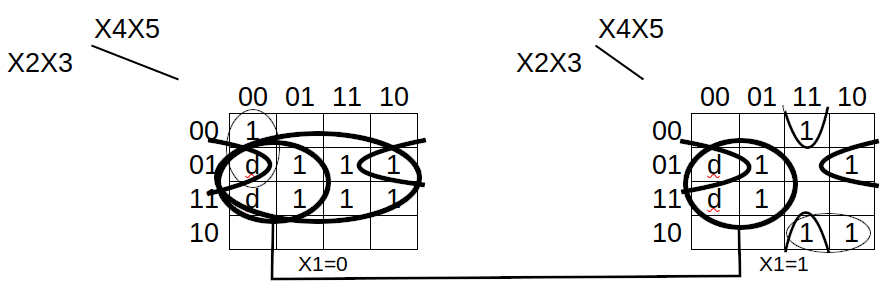
\includegraphics[width=\linewidth]{imgs/mdnf_karno.png}
\end{center}


\begin{equation*}
  \text{Получаем:}\hspace{1.5cm} C_{min}(f)= 
  \begin{Bmatrix}
    0 & X & 1 & X & X \\
    X & X & 1 & 0 & X \\
    X & 0 & 1 & X & 0 \\ 
    0 & 0 & X & 0 & 0 \\ 
    1 & X & 0 & 1 & 1 \\ 
    1 & 1 & 0 & 1 & X 
  \end{Bmatrix}
  \begin{pmatrix}
    1 \\ 2 \\ 3 \\ 4 \\ 5 \\ 6
  \end{pmatrix}
  S^a = 19; \hspace{0.5cm} S^b = 25
\end{equation*}

Отметим, что цены минимальных покрытий, полученных методом Квайна – 
Мак-Класки и с помощью карт Карно, совпадают, так как цена минимального 
покрытия булевой функции не зависит от метода его нахождения \\

МДНФ имеет следующий вид: \\
$ f = \
\nx{1}\x{3} \vee \
\x{3}\nx{4} \vee \
\nx{2}\x{3}\nx{5} \vee \
\nx{1}\nx{2}\nx{4}\nx{5} \vee \
\x{1}\nx{3}\x{4}\x{5}  \vee \
\x{1}\x{2}\nx{3}\x{4} \
$


\subsubsection{Определение МКНФ}

Получение МКНФ производится по нулевому покрытию булевой функции. 
Для этой цели на карте Карно выделяются клетки, соответствующие наборам 
аргументов,  на  которых  функция  принимает  нулевое  значение  (клетки 
отмечаются нулем). \\

\begin{center}
  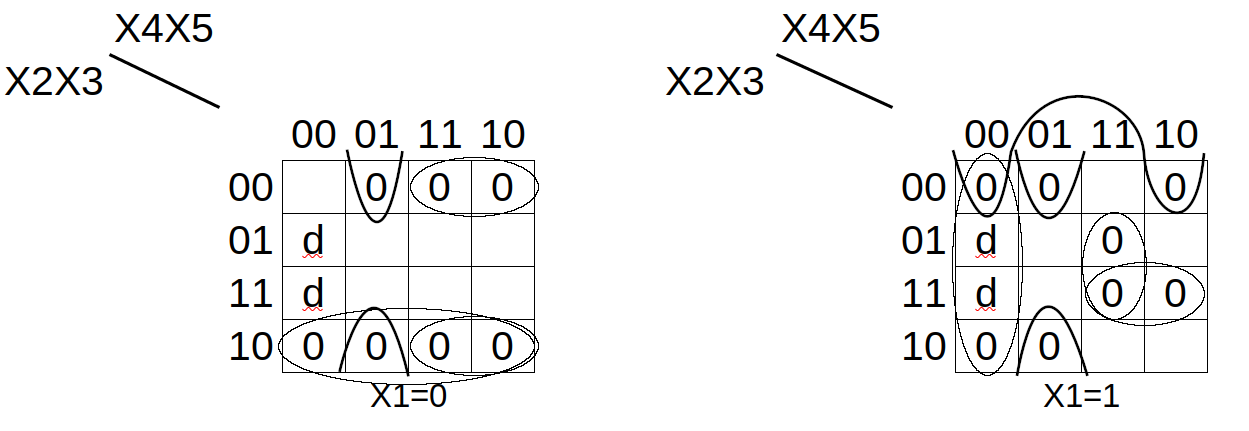
\includegraphics[width=\linewidth]{imgs/mknf_karno.png}
\end{center}

\begin{equation*}
  \text{Получаем:}\hspace{1.5cm} C_{min}(f)= 
  \begin{Bmatrix}
    0& 1& 0& X& X \\
    X& X& 0& 0& 1 \\
    0& X& 0& 1& X \\
    1& X& X& 0& 0 \\
    1& X& 1& 1& 1 \\
    1& 1& 1& 1& X \\
    1& 0& 0& X& 0 
  \end{Bmatrix}
  \begin{pmatrix}
    1 \\ 2 \\ 3 \\ 4 \\ 5 \\ 6
  \end{pmatrix}
  S^a = 24; \hspace{.5cm} S^b = 30
\end{equation*}

МКНФ : $f = \ 
(\x{1} \vee \nx{2} \vee \x{3}) \cdot \
(\x{3} \vee \x{4} \vee \nx{5}) \cdot \
(\x{1} \vee \x{3} \vee \nx{4}) \cdot \
(\nx{1} \vee \x{4} \vee \x{5}) \cdot \
(\nx{1} \vee \nx{3} \vee \nx{4} \vee \nx{5}) \cdot \
(\nx{1} \vee \x{2} \vee \x{3} \vee \x{5})\cdot \
(\nx{1} \vee \nx{2} \vee \nx{3} \vee \nx{4})\
$
\subsection{Преобразование минимальных форм булевой функции}
\textbf{Факторное преобразование для МДНФ:}

МДНФ : $ f = \
\nx{1}\x{3} \vee \
\x{3}\nx{4} \vee \
\nx{2}\x{3}\nx{5} \vee \
\nx{1}\nx{2}\nx{4}\nx{5} \vee \
\x{1}\nx{3}\x{4}\x{5}  \vee \
\x{1}\x{2}\nx{3}\x{4} \hspace{0.5cm} (S_Q = 25) \\ \   % Sq = 25
=  \
\x{3}(\nx{1} \vee \nx{4}) \vee \nx{2}\nx{5}(\x{3} \vee \nx{1}\nx{4}) \vee \ 
\x{1}\nx{3}\x{4}(\x{5} \vee \x{2})  \hspace{0.5cm} (S_Q = 20)
$
% 4 + (3+4) + (4 + 2)    + 3 = Sq = 20
\\

\textbf{Факторное преобразование для МКНФ:}

МКНФ : $f = \ 
(\x{1} \vee \nx{2} \vee \x{3}) \cdot \
(\x{3} \vee \x{4} \vee \nx{5}) \cdot \
(\x{1} \vee \x{3} \vee \nx{4}) \cdot \
(\nx{1} \vee \x{4} \vee \x{5}) \cdot \
(\nx{1} \vee \nx{3} \vee \nx{4} \vee \nx{5}) \cdot \
(\nx{1} \vee \x{2} \vee \x{3} \vee \x{5})\cdot \
(\nx{1} \vee \nx{2} \vee \nx{3} \vee \nx{4}) \hspace{0.5cm} (S_Q = 31)\\ \  % Sq = 31
= \
(\x{1}\vee\x{3}\vee\nx{2}\x{4})(\nx{1}\vee(\x{5}\vee(\x{4}(\x{2}\vee\x{3})))(\nx{3}\vee\nx{4}\vee\nx{2}\nx{3})) \hspace{0.5cm} (S_Q = 24)
$  % Sq = 24
\\

\par Решим задачу  декомпозиции  применительно  к  полученной  форме. 
Для этого введем вспомогательную функцию:

$
\phi = \phi(\x{2},\x{3})= \nx{2}\nx{3} \rightarrow \nphi = \x{2} \vee \x{3} \\
f = (\x{1}\vee\x{3}\vee\nx{2}\x{4})(\nx{1}\vee(\x{5}\vee(\x{4}\nphi))(\nx{3} \vee \nx{4} \vee \phi)) \hspace{0.5cm} (S_Q = 22)(2)
$
\subsection{Синтез комбинационных схем в булевом базисе}
Комбинационная схема, реализующая заданную функцию по аналитической 
форме (2), в булевом базисе с парафазными входами представлена  на  рисунке: 
\subsection{Синтез комбинационных схем в универсальных базисах}
\begin{center}
  \textbf{Базис(ИЛИ-НЕ)}
\end{center}

Приведение аналитического выражения (2) к базису (ИЛИ-НЕ) осуществляется заменой операций булева базиса на операцию стрелка Пирса (отрицание дизъюнкции) путем использования законов двойственности. 

$
\phi = \nx{2}\nx{3}= \overline{\overline{\nx{2}\nx{3}}}= \overline{\pirs{\nx{2}}{\nx{3}}} \rightarrow \nphi = \pirs{\nx{2}}{\nx{3}} 
$

\begin{align*}
f &= (\x{1}\vee\x{3}\vee\nx{2}\x{4})(\nx{1}\vee(\x{5}\vee\x{4}\nphi)(\nx{3} \vee \nx{4} \vee \phi)) = \\
  &=\neg{ \x{1}\vee\x{3}\vee \neg{\x{2}\vee\nx{4}} }
    \vee
    \neg{
      \nx{1} \vee
      \neg{ \x{5} \vee \neg{\nx{4}\vee\phi}} \vee
      \neg{ \nx{3} \vee \nx{4} \vee \phi   }
    } = \\
  &=(\x{1}\downarrow\x{3}\downarrow (\x{2}\downarrow\nx{4}))
    \downarrow
    (\nx{1} \downarrow
      (\x{5} \downarrow (\nx{4}\downarrow\phi)) 
      \downarrow
      (\nx{3} \downarrow \nx{4} \downarrow \phi)
    )
\end{align*}

По полученному выражению строим схему с парафазными входами в базисе (ИЛИ-НЕ):
% \begin{center}
% \includegraphics[width=\linewidth]{imgs/circuit-ornot_basis.png}
% \end{center}

\end{document}